% -*- coding: utf-8 -*-
%-------------------------designed by zcf--------------
\documentclass[UTF8,a4paper,10pt]{ctexart}
\usepackage[left=3.17cm, right=3.17cm, top=2.74cm, bottom=2.74cm]{geometry}
\usepackage{amsmath}
\usepackage{graphicx,subfig}
\usepackage{float}
\usepackage{cite}
\usepackage{caption}
\usepackage{enumerate}
\usepackage{booktabs} %表格
\usepackage{multirow}
\usepackage{pythonhighlight}
\newcommand{\tabincell}[2]{\begin{tabular}{@{}#1@{}}#2\end{tabular}}  %表格强制换行
%-------------------------字体设置--------------
\usepackage{times} 
\newcommand{\yihao}{\fontsize{26pt}{36pt}\selectfont}           % 一号, 1.4 倍行距
\newcommand{\erhao}{\fontsize{22pt}{28pt}\selectfont}          % 二号, 1.25倍行距
\newcommand{\xiaoer}{\fontsize{18pt}{18pt}\selectfont}          % 小二, 单倍行距
\newcommand{\sanhao}{\fontsize{16pt}{24pt}\selectfont}  %三号字
\newcommand{\xiaosan}{\fontsize{15pt}{22pt}\selectfont}        % 小三, 1.5倍行距
\newcommand{\sihao}{\fontsize{14pt}{21pt}\selectfont}            % 四号, 1.5 倍行距
\newcommand{\banxiaosi}{\fontsize{13pt}{19.5pt}\selectfont}    % 半小四, 1.5倍行距
\newcommand{\xiaosi}{\fontsize{12pt}{18pt}\selectfont}            % 小四, 1.5倍行距
\newcommand{\dawuhao}{\fontsize{11pt}{11pt}\selectfont}       % 大五号, 单倍行距
\newcommand{\wuhao}{\fontsize{10.5pt}{15.75pt}\selectfont}    % 五号, 单倍行距
%-------------------------章节名----------------
\usepackage{ctexcap} 
\CTEXsetup[name={,、},number={ \chinese{section}}]{section}
\CTEXsetup[name={(,)},number={\chinese{subsection}}]{subsection}
\CTEXsetup[name={,.},number={\arabic{subsubsection}}]{subsubsection}
%-------------------------页眉页脚--------------
\usepackage{fancyhdr}
\pagestyle{fancy}
\lhead{\kaishu \leftmark}
% \chead{}
\rhead{\kaishu 机器学习实验报告}%加粗\bfseries 
\lfoot{}
\cfoot{\thepage}
\rfoot{}
\renewcommand{\headrulewidth}{0.1pt}  
\renewcommand{\footrulewidth}{0pt}%去掉横线
\newcommand{\HRule}{\rule{\linewidth}{0.5mm}}%标题横线
\newcommand{\HRulegrossa}{\rule{\linewidth}{1.2mm}}
%-----------------------伪代码------------------
\usepackage{algorithm}  
\usepackage{algorithmicx}  
\usepackage{algpseudocode}  
\floatname{algorithm}{Algorithm}  
\renewcommand{\algorithmicrequire}{\textbf{Input:}}  
\renewcommand{\algorithmicensure}{\textbf{Output:}} 
\usepackage{lipsum}  
\makeatletter
\newenvironment{breakablealgorithm}
  {% \begin{breakablealgorithm}
  \begin{center}
     \refstepcounter{algorithm}% New algorithm
     \hrule height.8pt depth0pt \kern2pt% \@fs@pre for \@fs@ruled
     \renewcommand{\caption}[2][\relax]{% Make a new \caption
      {\raggedright\textbf{\ALG@name~\thealgorithm} ##2\par}%
      \ifx\relax##1\relax % #1 is \relax
         \addcontentsline{loa}{algorithm}{\protect\numberline{\thealgorithm}##2}%
      \else % #1 is not \relax
         \addcontentsline{loa}{algorithm}{\protect\numberline{\thealgorithm}##1}%
      \fi
      \kern2pt\hrule\kern2pt
     }
  }{% \end{breakablealgorithm}
     \kern2pt\hrule\relax% \@fs@post for \@fs@ruled
  \end{center}
  }
\makeatother
%------------------------代码-------------------
\usepackage{xcolor} 
\usepackage{listings} 
\lstset{ 
breaklines,%自动换行
basicstyle=\small,
escapeinside=``,
keywordstyle=\color{ blue!70} \bfseries,
commentstyle=\color{red!50!green!50!blue!50},% 
stringstyle=\ttfamily,% 
extendedchars=false,% 
linewidth=\textwidth,% 
numbers=left,% 
numberstyle=\tiny \color{blue!50},% 
frame=trbl% 
rulesepcolor= \color{ red!20!green!20!blue!20} 
}
%------------超链接----------
\usepackage[colorlinks,linkcolor=black,anchorcolor=blue]{hyperref}
%------------------------TODO-------------------
\usepackage{enumitem,amssymb}
\newlist{todolist}{itemize}{2}
\setlist[todolist]{label=$\square$}
% for check symbol 
\usepackage{pifont}
\newcommand{\cmark}{\ding{51}}%
\newcommand{\xmark}{\ding{55}}%
\newcommand{\done}{\rlap{$\square$}{\raisebox{2pt}{\large\hspace{1pt}\cmark}}\hspace{-2.5pt}}
\newcommand{\wontfix}{\rlap{$\square$}{\large\hspace{1pt}\xmark}}
%------------------------水印-------------------
\usepackage{tikz}
\usepackage{xcolor}
\usepackage{eso-pic}

\newcommand{\watermark}[3]{\AddToShipoutPictureBG{
\parbox[b][\paperheight]{\paperwidth}{
\vfill%
\centering%
\tikz[remember picture, overlay]%
  \node [rotate = #1, scale = #2] at (current page.center)%
    {\textcolor{gray!80!cyan!30!magenta!30}{#3}};
\vfill}}}



%———————————————————————————————————————————正文———————————————————————————————————————————————
%----------------------------------------------
\begin{document}
\begin{titlepage}
    \begin{center}
    
\includegraphics[width=0.8\textwidth]{NKU.png}\\[1cm]    
    \textsc{\Huge \kaishu{\textbf{南\ \ \ \ \ \ 开\ \ \ \ \ \ 大\ \ \ \ \ \ 学}} }\\[0.9cm]
    \textsc{\huge \kaishu{\textbf{计\ \ 算\ \ 机\ \ 学\ \ 院}}}\\[0.5cm]
    \textsc{\Large \textbf{机器学习实验报告}}\\[0.8cm]
    \HRule \\[0.9cm]
    { \LARGE \bfseries 实验四\ 朴素贝叶斯分类器}\\[0.4cm]
    \HRule \\[2.0cm]
    \centering
    \textsc{\LARGE \kaishu{姓名\ :\ 王泳鑫}}\\[0.5cm]
    \textsc{\LARGE \kaishu{学号\ :\ 1911479}}\\[0.5cm]
    \textsc{\LARGE \kaishu{年级\ :\ 2019级}}\\[0.5cm]
    \textsc{\LARGE \kaishu{专业\ :\ 计算机科学与技术}}\\[0.5cm]
    \textsc{\LARGE \kaishu{指导教师\ :\ 卫金茂}}\\[0.5cm]
    \vfill
    {\Large \today}
    \end{center}
\end{titlepage}
%-------------摘------要--------------
\newpage
\thispagestyle{empty}
\renewcommand{\abstractname}{\kaishu \sihao \textbf{摘要}}
    \begin{abstract}

        \noindent  %顶格
        \textbf{\\\ 关键字:朴素贝叶斯,Machine Learning , Deep Learning}\textbf{} \\\ \\\
    \end{abstract}
%----------------------------------------------------------------
\tableofcontents
%----------------------------------------------------------------
\newpage
\watermark{60}{10}{NKU}
\setcounter{page}{1}
%——————————————————————————————————————
\section{实验描述}
\subsection{实验内容}
Most Popular Data Set中的wine数据集(对意大利同一地区声场的三种不同品种的酒做大量分析所得出的数据)

\subsection{实验要求}


基本要求:

\begin{itemize}
   \item 采用分层采样的方式将数据集划分为训练集和测试集。 
   \item 给定编写一个朴素贝叶斯分类器,对测试集进行预测,计算分类准确率。
\end{itemize}

中级要求:

\begin{itemize}
   \item 使用测试集评估模型,得到混淆矩阵,精度,召回率,F值。
\end{itemize}



%——————————————————————————————————————
\section{代码实现}

首先时读取数据的部分,通过numpy库的loadtxt读取数据,并且遍历数据集,将不同类别的数据放入三个list中,返回这三个列表。

\begin{python}
   # 读取数据
   def read_data(path):
       data = list(np.loadtxt(path, delimiter=','))
       # 打乱数据,为方便训练集和测试集划分
       random.shuffle(data)
       data = np.array(data)
       sample1 = []
       sample2 = []
       sample3 = []
       for each in data:
           if each[0] == 1:
               sample1.append(each)
           elif each[0] == 2:
               sample2.append(each)
           else:
               sample3.append(each)
       return np.array(sample1), np.array(sample2), np.array(sample3)

\end{python}

然后我们要对数据集进行一个划分,基本要求中写到,需要采用分层抽样的的方法划分训练集和测试集,
先将所有个体样本按照某种特征划分为几个类别,这一步我们在读取数据的函数中已经实现了,
然后从每个类别中使用随机抽样或等距抽样的方法选择个体组成样本。

\begin{python}
   def train_test_split(sample1, sample2, sample3, fold, idx):
    train_sample1 = []
    train_sample2 = []
    train_sample3 = []
    test_sample = []
    for i in range(sample1.shape[0]):
        if i % fold != idx:
            train_sample1.append(sample1[i])
        else:
            test_sample.append(sample1[i])
    for i in range(sample2.shape[0]):
        if i % fold != idx:
            train_sample2.append(sample2[i])
        else:
            test_sample.append(sample2[i])
    for i in range(sample3.shape[0]):
        if i % fold != idx:
            train_sample3.append(sample3[i])
        else:
            test_sample.append(sample3[i])
    train_sample1 = np.array(train_sample1)
    train_sample2 = np.array(train_sample2)
    train_sample3 = np.array(train_sample3)
    train_label1 = train_sample1[:, 0]
    train_label2 = train_sample2[:, 0]
    train_label3 = train_sample3[:, 0]
    train_sample1 = train_sample1[:, 1:]
    train_sample2 = train_sample2[:, 1:]
    train_sample3 = train_sample3[:, 1:]
    test_sample = np.array(test_sample)
    test_label = test_sample[:, 0]
    test_sample = test_sample[:, 1:]
    return train_sample1, train_label1, train_sample2, train_label2, \
           train_sample3, train_label3, test_sample, test_label
\end{python}

接下来我们需要计算极大后验概率,公式如下:

\begin{equation}
    c_{M A P}=\operatorname{argmax}_{\mathrm{c}_{k} \in C} P\left(c_{k} \mid x\right)=\operatorname{argmax}_{c_{k} \in C} \frac{P\left(x \mid c_{k}\right) P\left(c_{k}\right)}{P(x)}=\operatorname{argmax}_{c_{k} \in C} P\left(x \mid c_{k}\right) P\left(c_{k}\right)
\end{equation}

\begin{python}
   def cal_para(sample):
    mean = np.mean(sample, 0)
    var = np.var(sample, 0)
    return mean, var


def cal_prob(test_vec, train_sample, total):
    mean, var = cal_para(train_sample)
    # 根据高斯函数计算
    prob = (1 / np.sqrt(2*np.pi*var)) * np.exp(-np.square(test_vec - mean) / (2*var))
    # 先验概率
    prior = train_sample.shape[0] / total
    likelihood = 1
    for each in prob:
        # 连乘条件概率
        likelihood *= each
    return prior*likelihood
\end{python}

然后是预测标签的函数,通过上面的计算概率函数,选择概率最大的作为预测标签,代码如下:

\begin{python}
    def decide_label(test_sample, train_sample1, train_sample2, train_sample3):
    total = train_sample1.shape[0] + train_sample2.shape[0] + train_sample3.shape[0]
    label = []
    score = []
    for each in test_sample:
        prob1 = cal_prob(each, train_sample1, total)
        prob2 = cal_prob(each, train_sample2, total)
        prob3 = cal_prob(each, train_sample3, total)
        # 选择概率最大的作为预测标签
        if max([prob1, prob2, prob3]) == prob1:
            label.append(1)
        elif max([prob1, prob2, prob3]) == prob2:
            label.append(2)
        else:
            label.append(3)
        score.append(prob1)
    return np.array(label), np.array(score)

\end{python}

下面则是本次实验交叉验证的函数,参数sample分别是对应数据集中的三个类别,fold代表折数

\begin{python}
def cross_valid(sample1, sample2, sample3, fold):
    acc = []
    for i in range(fold):
        train_sample1, train_label1, train_sample2, train_label2, \
        train_sample3, train_label3, \
        test_sample, test_label = train_test_split(sample1, sample2, sample3, fold, i)
        pred_label, pred_score = decide_label(test_sample, train_sample1, train_sample2, train_sample3)
        correct = 0
        for j in range(test_label.shape[0]):
            if pred_label[j] == test_label[j]:
                correct += 1
        print(i, 'acc:', correct / test_label.shape[0])
        acc.append(correct / test_label.shape[0])
    return np.mean(acc)
\end{python}

后面,是提高要求的部分,我们可以通过下面结果分析的函数来构造混淆矩阵,精度,召回率和F值,这一部分只要根据公式就可以顺利地写出来:


\begin{python}
    def result_analysis(sample1, sample2, sample3):
    train_sample1, train_label1, train_sample2, train_label2, \
    train_sample3, train_label3, \
    test_sample, test_label = train_test_split(sample1, sample2, sample3, fold, 1)
    pred_label, pred_score = decide_label(test_sample, train_sample1, train_sample2, train_sample3)
    cm = np.zeros((3, 3))
    # 构造混淆矩阵
    for i in range(test_label.shape[0]):
        cm[int(test_label[i]) - 1, pred_label[i] - 1] += 1
    tp1 = cm[0, 0]
    tp2 = cm[1, 1]
    tp3 = cm[2, 2]
    fn1 = cm[0, 1] + cm[0, 2]
    fn2 = cm[1, 0] + cm[1, 2]
    fn3 = cm[2, 0] + cm[2, 1]
    fp1 = cm[1, 0] + cm[2, 0]
    fp2 = cm[0, 1] + cm[2, 1]
    fp3 = cm[0, 2] + cm[1, 2]
    tn1 = cm[1, 1] + cm[1, 2] + cm[2, 1] + cm[2, 2]
    tn2 = cm[0, 0] + cm[0, 2] + cm[2, 0] + cm[2, 2]
    tn3 = cm[0, 0] + cm[0, 1] + cm[1, 0] + cm[1, 1]
    # 根据公式计算precision、recall和F1
    precision1 = tp1 / (tp1 + fp1)
    precision2 = tp2 / (tp2 + fp2)
    precision3 = tp3 / (tp3 + fp3)
    recall1 = tp1 / (tp1 + fn1)
    recall2 = tp2 / (tp2 + fn2)
    recall3 = tp3 / (tp3 + fn3)
    f1 = (2*precision1*recall1) / (precision1 + recall1)
    f2 = (2*precision2*recall2) / (precision2 + recall2)
    f3 = (2*precision3*recall3) / (precision3 + recall3)
    return cm, precision1, precision2, precision3, recall1, recall2, recall3, f1, f2, f3
\end{python}
%——————————————————————————————————————
\section{实验结果展示与分析}

对于交叉验证,我们得到的结果如图\ref{fig:1}所示:

\begin{figure}[H]
    \centering
    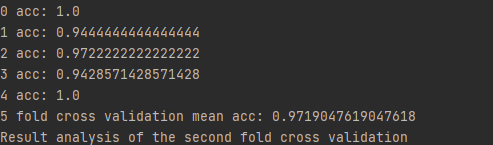
\includegraphics[scale=1]{1.png}
    \caption{交叉验证结果}
    \label{fig:1}
\end{figure}

我们可以看到5折交叉检验的平均准确率达到了0.9719,可以看到该分类器得到的分类结果可信度还是比较高。

根据公式我们得到的混淆矩阵如图\ref{fig:1}所示:

\begin{figure}[H]
    \centering
    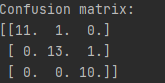
\includegraphics[scale=1]{2.png}
    \caption{混淆矩阵}
    \label{fig:1}
\end{figure}

经过result\_analysis函数的计算,我们得到的精度如下图\ref{fig:1}所示:

\begin{figure}[H]
    \centering
    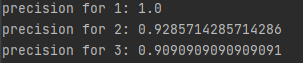
\includegraphics[scale=1]{3.png}
    \caption{精度}
    \label{fig:1}
\end{figure}

召回率如下图\ref{fig:1}所示:

\begin{figure}[H]
    \centering
    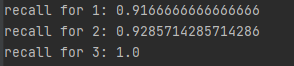
\includegraphics[scale=1]{4.png}
    \caption{召回率}
    \label{fig:1}
\end{figure}

F如下图\ref{fig:1}所示:

\begin{figure}[H]
    \centering
    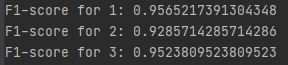
\includegraphics[scale=1]{5.png}
    \caption{F值}
    \label{fig:1}
\end{figure}

%----------------------------------------------------------------

%----------------------------------------------------------------
\bibliographystyle{plain}
\end{document}
